
% This LaTeX was auto-generated from MATLAB code.
% To make changes, update the MATLAB code and republish this document.

\documentclass{article}
\usepackage{graphicx}
\usepackage{color}

\sloppy
\definecolor{lightgray}{gray}{0.5}
\setlength{\parindent}{0pt}

\begin{document}

    
    
\section*{ODE Mini-Report Assignment (By Patrice Harapeti)}


\subsection*{Contents}

\begin{itemize}
\setlength{\itemsep}{-1ex}
   \item Background
   \item Part Zero : Setup
   \item Part One : Analytical Solution
   \item Part Two : Exploration of Analytical Solution
   \item Part Three : Numerical Solution (TODO USE EULERS OR ANOTHER METHOD)
   \item Part Four : Analyis of error with varying step size
   \item Part Five : Fourier Analysis of numerical solution
   \item Part Six : Function Definitions
\end{itemize}


\subsection*{Background}

\begin{par}
Simple Damped Oscillator
\end{par} \vspace{1em}
\begin{verbatim}
% Discuss a damped oscillator and it's features

% Identify the oscillation frequency and maximum amplitude

% Display master equation and how the analytical solution is derived

% Display how and why Euler's method is used to numerically solve the PDE

% Explore analytical solution with varying parameters and discuss the three
% cases (underdamped, critically damped, overdamped)

% Determine error between analytical and numerical based on changing step
% size

% Perform Fourier Analysis of a particular case of the analytical solution

% Discuss FWHM and frequency (compare this with calculated oscillation
% frequency from above)
\end{verbatim}


\subsection*{Part Zero : Setup}

\begin{verbatim}
% Clear existing workspace
clear; clc; close all

% Setup parameters
timestep = 0.01; % timestep (seconds)
totalTime = 100; % total time of simulation (seconds)
timeSeries = 0:timestep:totalTime;

% Define initial conditions of system
x_initial = 2; % initial position (metres)
v_initial = 0; % intial velocity (metres / second)
\end{verbatim}


\subsection*{Part One : Analytical Solution}

\begin{verbatim}
% Plot analytical solution
figure('NumberTitle', 'off', 'Name', 'Analytical Solution of each case');
yline(0, '--');
grid on;

% Overdamped case
plot(timeSeries, generateAnalyticalSolution(timeSeries, 2, 0.1, x_initial));
hold on;

% Critically Damped case
plot(timeSeries, generateAnalyticalSolution(timeSeries, 2, 1, x_initial), 'g');
hold on;

% Underdamped case
plot(timeSeries, generateAnalyticalSolution(timeSeries, 1, 5, x_initial), 'r');
title('Analytical Solution');
xlabel('Time');
ylabel('Position');
legend('Overdamped', 'Critically Damped', 'Underdamped');
hold off;
\end{verbatim}

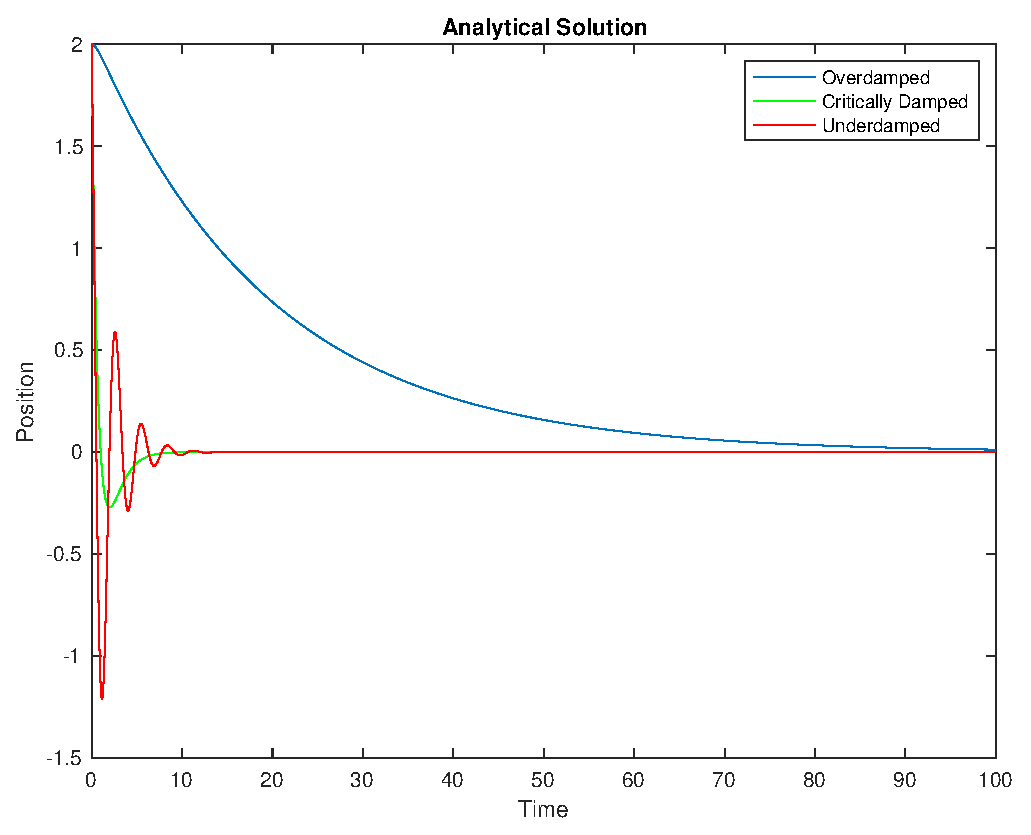
\includegraphics [width=4in]{ode_mini_report_01.eps}


\subsection*{Part Two : Exploration of Analytical Solution}

\begin{par}
Plot surface plot of gamma/k vs time to visualise how the ratio (dampening) of the parameters affect the function
\end{par} \vspace{1em}
\begin{verbatim}
% Fix value of parameter k while gamma changes
kExplore = 1;

% Determine number of points required in discretization
noPoints = 100;

timeSeries = linspace(0, totalTime, noPoints);
gammaSeries = linspace(0, 2, noPoints);
ratioSeries = nan(size(gammaSeries));
positionSeries = nan(size(gammaSeries));

% Build up vectors
for i = 1:length(gammaSeries)
    % Calculate gamma using kExplore
    gamma = gammaSeries(i);

    % Calculate ratio using gamma and kExplore
    ratioSeries(i) = gamma.^2 ./ kExplore;

    % Calculate position based on time and gamma ratio
    positionSeries(i, :) = generateAnalyticalSolution(timeSeries, gamma, kExplore, x_initial);
end

% Plot ratio of parameters vs position and time
figure('NumberTitle', 'off', 'Name', 'Function Behavioural Analysis');
surf(timeSeries, ratioSeries, positionSeries);

% Decorate surface plot
colorbar
title('Behaviour of anaytical solution')
xlabel('Gamma squared / k = 4 ratio');
ylabel('Time (s)');
zlabel('Position (m)');

% Adjust camera viewport
%view([-15 3 4]);
\end{verbatim}

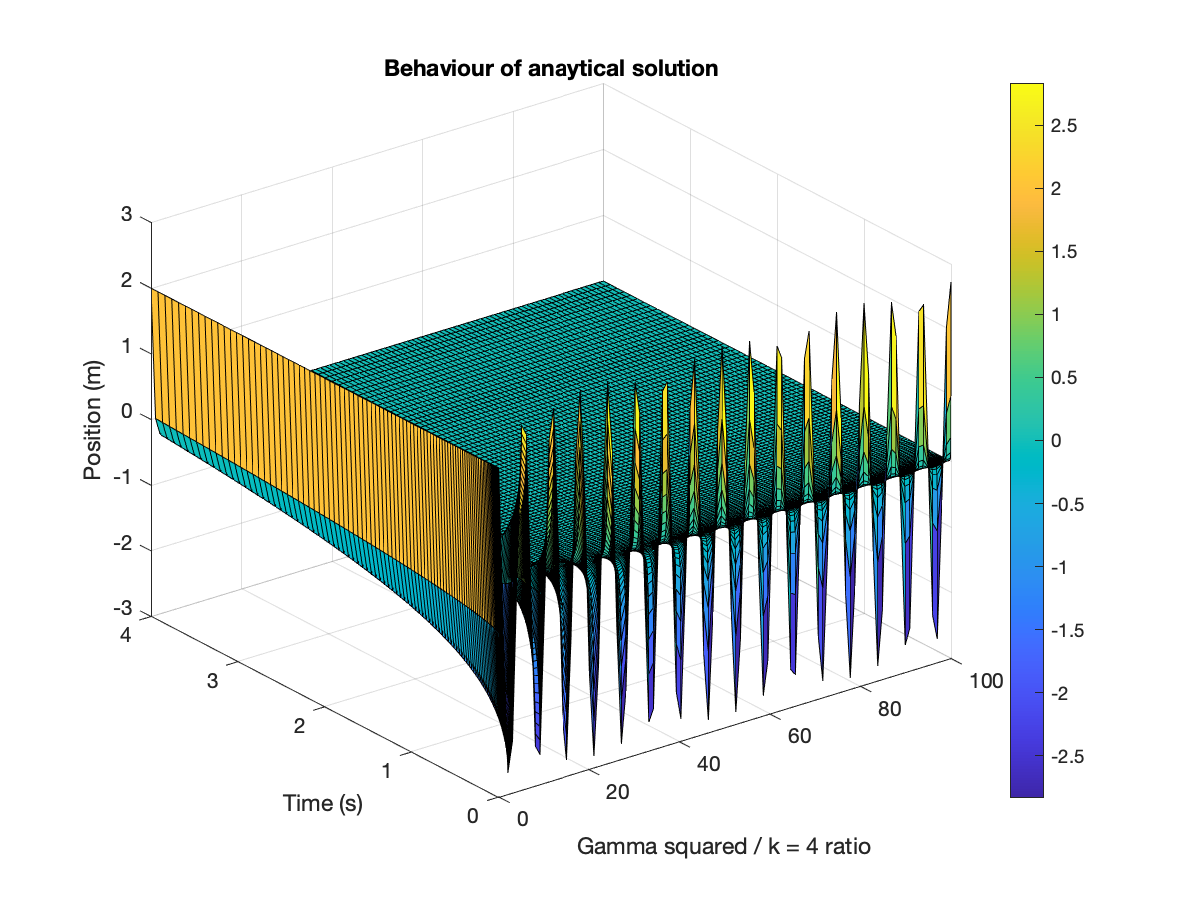
\includegraphics [width=4in]{ode_mini_report_02.eps}


\subsection*{Part Three : Numerical Solution (TODO USE EULERS OR ANOTHER METHOD)}

\begin{verbatim}
% Generate numerical solution for the underdamped case
[numerical_position, numerical_velocity] = generateNumericalSolution(timeSeries, 0.5, 2, x_initial, v_initial);

% Plot Position vs Time
figure('NumberTitle', 'off', 'Name', 'Numerical Solution of underdamped case');
subplot(1, 3, 1);
plot(timeSeries, numerical_position);

% Draw horizontal line at y = 0 to represent convergence value
yline(0, '--');
grid on;
title('Position vs Time');
xlim([0, 70]);
xlabel('Time (s)');
ylabel('Position (m)');

% Plot Velocity vs Time
subplot(1, 3, 2);
plot(timeSeries, numerical_velocity, 'r');
grid on;
title('Velocity vs Time');
xlim([0, 70]);
xlabel('Time (s)');
ylabel('Velocity (m/s)');

% Plot Position vs Velocity
subplot(1, 3, 3);
plot(numerical_position, numerical_velocity, 'g', 'LineWidth', 1.2);
grid on;
title('Postion vs Velocity');
xlabel('Position (m)');
ylabel('Velocity (m/s)');
\end{verbatim}

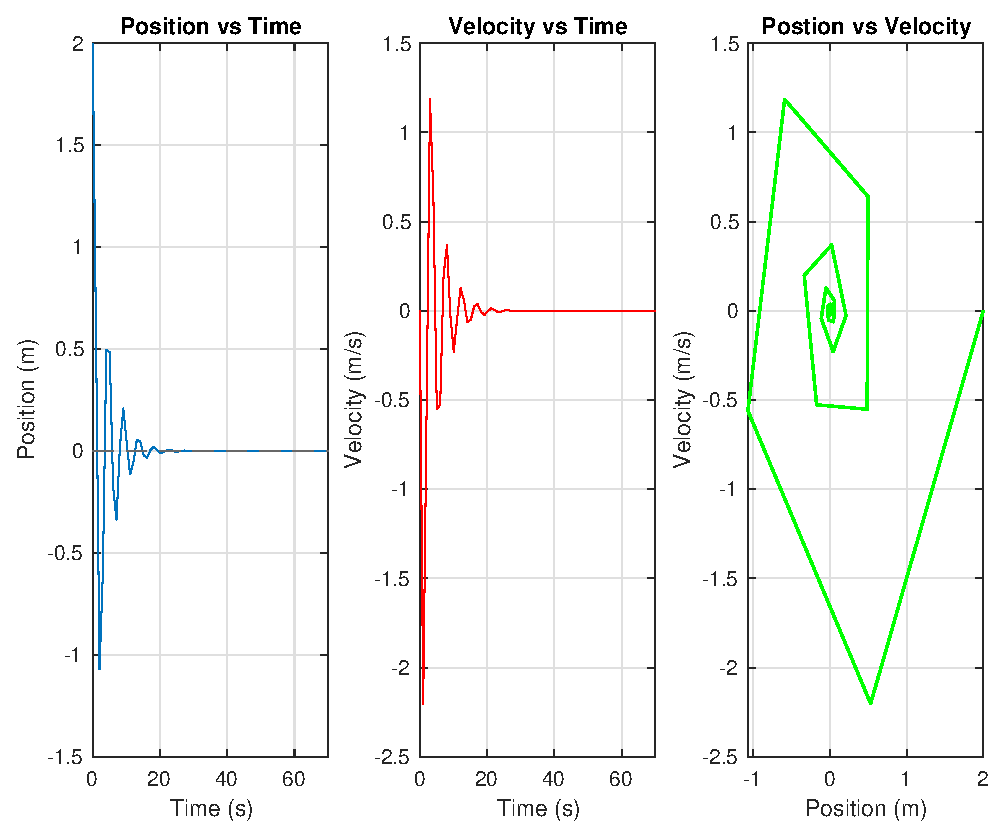
\includegraphics [width=4in]{ode_mini_report_03.eps}


\subsection*{Part Four : Analyis of error with varying step size}

\begin{verbatim}
% Pick particular case, underdamped in this case
gammaErrorAnalysis = 0.1;
kErrorAnalysis = 3;

% Generate range of step sizes
stepSizes = linspace(0.001, 1);
averageErrorAtStepSize = nan(size(stepSizes));
relativePercentErrorAtStepSize = nan(size(stepSizes));

% Loop over each discretized step size
for i = 1:length(stepSizes)
    % Generate timeseries for discretized total time based on step size
    varyingTimeSeries = 0:stepSizes(i):totalTime;

    % Generate analytical solution with timeseries
    analyticalPos = generateAnalyticalSolution(varyingTimeSeries, gammaErrorAnalysis, kErrorAnalysis, x_initial);

    % Generate numerical solution with same timeseries
    [numericalPos, ~] = generateNumericalSolution(varyingTimeSeries, gammaErrorAnalysis, kErrorAnalysis, x_initial, v_initial);

    % Calculate error at the current step size
    [averageError, relativeError] = calculateError(analyticalPos, numericalPos.');
    averageErrorAtStepSize(i) = averageError;
    relativePercentErrorAtStepSize(i) = relativeError .* 100;
end

% Plot each type of error vs step size
% We expect the error to be reduced as the step size is minimised
figure('NumberTitle', 'off', 'Name', 'Error Analysis');
subplot(1, 2, 1);
loglog(stepSizes, averageErrorAtStepSize);
title('Average Error vs Step Size');
xlabel('Step Size (log)');
ylabel('Average Error');
legend('Average Error');

subplot(1, 2, 2);
loglog(stepSizes, relativePercentErrorAtStepSize, 'r');
title('Relative Error (%) vs Step Size');
xlabel('Step Size (log)');
ylabel('Relative Error (%)');
legend('Relative Error (%)');
\end{verbatim}

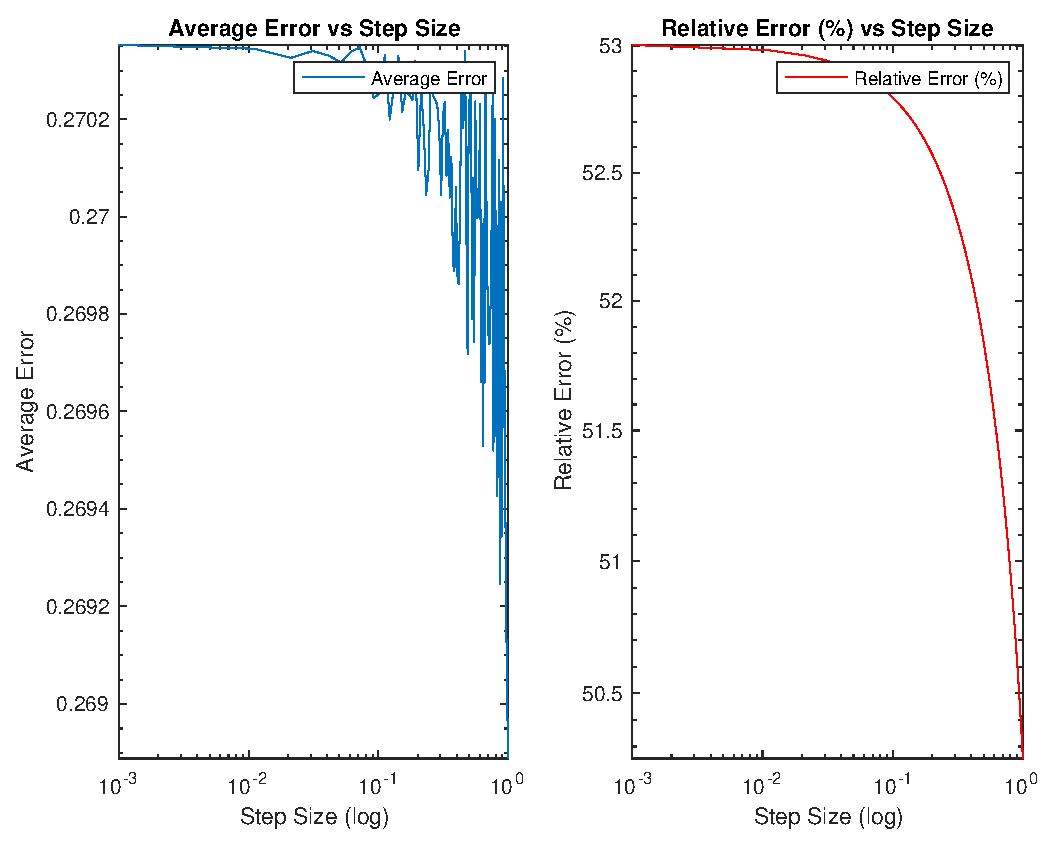
\includegraphics [width=4in]{ode_mini_report_04.eps}


\subsection*{Part Five : Fourier Analysis of numerical solution}

\begin{verbatim}
% Determine equation parameters for the underdamped case
gammaFourier = 0.5;
kFourier = 2;

% Generate positions of analytical solution
analytical_position = generateAnalyticalSolution(timeSeries, gammaFourier, kFourier, x_initial);

% Define new domain to transformed into frequency space
x = linspace(-1,1,length(timeSeries)).' * 10;
power_real = abs(analytical_position).^2;

% Plot real power of analytical solution vs x
figure('NumberTitle', 'off', 'Name', 'Fourier Analysis of critically damped case');
subplot(1, 3, 1);
plot(x, power_real, 'Color','#008000');
title('Power vs x');
xlim([-3, 3]);
xlabel('x');
ylabel('Power');
legend('Power');

% Perform Fast Fourier Transform on Analytical Solution
N = length(x); % Number of samples
Y = fft(analytical_position); % Compute Fast Fourier Transformation
dx = mean(diff(x)); % Determine sample spacing
df = 1/(N*dx); % Determine frequency spacing
fi = (0:(N-1)) - floor(N/2); % Generate unfolded index
frequency = df * fi; % Generate frequency vector
power_freq = abs(Y) .^ 2; % Calculate absolute power in frequency space

% Plot Power vs Frequency
subplot(1, 3, 2);
plot(frequency, power_freq);
title('Power vs Frequency');
xlabel('Hz');
ylabel('Power');
legend('Power');

% Limit power (in frequency domain) to be positive for frequency analysis
frequencyPositive = frequency .* (frequency > 0);
powerPositive = power_freq .* (power_freq > 0);

% Plot power (frequency domain) vs frequency for positive frequencies
subplot(1, 3, 3);
plot(frequencyPositive, powerPositive, '-r');
title('Power vs Frequency');
subtitle('For positive frequencies');
xlabel('Hz');
ylabel('Power');
legend('Power');
hold on;

% Estimate center frequency in frequency domain and include in plot
powerSum_freq = sum(powerPositive);
weightedPowerSum_freq = sum(powerPositive .* frequencyPositive.');
expectedCenterFrequency_freq = weightedPowerSum_freq ./ powerSum_freq;

% Determine FWHM and include in plot
\end{verbatim}


\subsection*{Part Six : Function Definitions}

\begin{verbatim}
function position = generateAnalyticalSolution(timeSeries, gamma, k, x_init)
    %   Derivation
    %   Let x = e^bt
    %   therefore... xdot = b * e^bt
    %   therefore... xddot = b^2 * e^bt
    %
    %   Plugging into the original PDE give us...
    %   -b^2 * e^bt - (gamma * b * e^bt) - ke^bt = 0
    %
    %   Pull e^bt out as common factor, this leaves us...
    %   e^bt (-b^2 - gamma*b - k) = 0
    %
    %   Therefore b^2 + gamma*b + k must equal 0
    %   Solving for b
    %   b = (gamma ± sqrt((gamma)^2 - (4k)) / -2
    %
    %   Overdamped when...         gamma^2 - 4k > 0
    %   Critically damped when...  gamma^2 - 4k = 0
    %   Underdamped when...        gamma^2 - 4k < 0

    % Calculate roots of characteristics equations
    b_1 = (-gamma + sqrt(gamma.^2 - (4 .* k))) ./ 2;
    b_2 = (-gamma - sqrt(gamma.^2 - (4 .* k))) ./ 2;

    % Define discriminant of characteristic equation
    discriminant = gamma.^2 - (4 .* k);

    % Define function in three cases based on the determinant of the roots
    % Reference: https://nrich.maths.org/11054
    if discriminant == 0 % critically damped
        % Solve for A and B constants
        A = x_init;
        B = x_init .* b_1;

        position = (A + B.*timeSeries) .* exp(b_1 .* timeSeries);
    elseif discriminant > 0 % overdamped
        % Solve for A and B constants
        A = (x_init .* b_2) ./ (b_2 - b_1);
        B = (x_init .* b_1) ./ (b_1 - b_2);

        position = (A .* exp(b_1 .* timeSeries)) + ...
            (B .* exp(b_2 .* timeSeries));

    else % underdamped if discriminant is less than 0
        % Separate real and imaginary parts of roots
        alpha = real(b_1);
        beta = imag(b_2);

        % Solve for A and B constants
        A = x_init;
        B = -x_init ./ beta;

        position = exp(alpha .* timeSeries) .* ...
            (A.*cos(beta.*timeSeries) + B.*sin(beta.*timeSeries));
    end
end

function [position, velocity] = generateNumericalSolution(timeSeries, gamma, k, x_initial, v_initial)
    % Negatively dampened (will converge at y = 0)
    % Also known as an underdamped system
    A = [0 1; -k -gamma];

    % Use ode45 to numerically solve system of equations
    [~, x] = ode45(@(t, x) A * x, timeSeries, [x_initial, v_initial]);
    position = x(:, 1);
    velocity = x(:, 2);
end

function [averageError, relativeError] = calculateError(analyticalSolution, numericalSolution)
    % Absolute error between analytical and numerical solution
    absoluteError = abs(analyticalSolution - numericalSolution);

    % Calculate Average Absolute Error
    % Reference: https://sutherland.che.utah.edu/wiki/index.php/Iteration_and_Convergence
    averageError = norm(absoluteError) ./ sqrt(length(analyticalSolution));

    % Calculate Relative Error
    relativeError = norm(absoluteError) ./ norm(abs(analyticalSolution));
end
\end{verbatim}



\end{document}

